
\begin{figure}
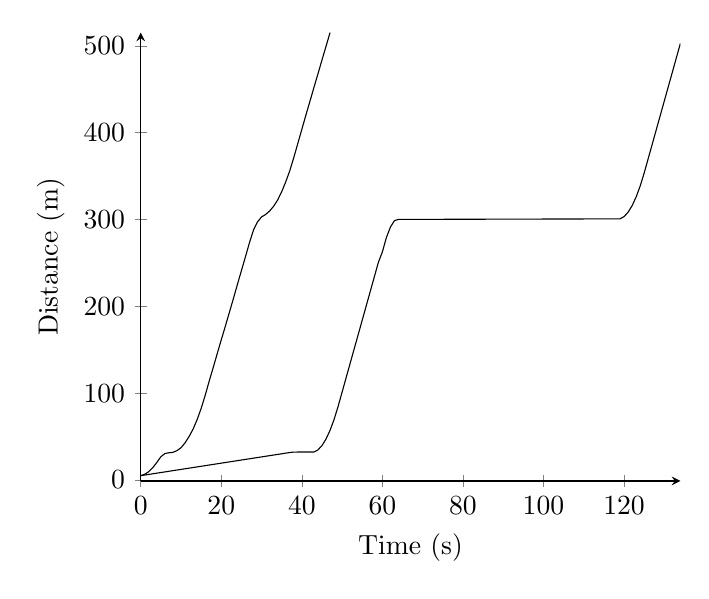
\begin{tikzpicture}
\begin{axis}[
legend style={
	anchor=west
},
axis x line=bottom,
axis y line=left,
ymin=-1,
point meta=explicit symbolic,
xlabel=Time (s),
ylabel=Distance (m)
]
\addplot[] coordinates {
(0, 5.1)
(1, 6.73988304033)
(2, 9.71703632929)
(3, 14.3804208174)
(4, 20.3417556429)
(5, 26.9337973525)
(6, 30.5670688723)
(7, 31.4435447984)
(8, 31.9685917306)
(9, 33.8876906473)
(10, 37.2908310737)
(11, 42.9022030701)
(12, 50.1485314453)
(13, 58.7528129048)
(14, 69.6428537233)
(15, 82.5838119337)
(16, 97.5483452172)
(17, 114.102592686)
(18, 129.751162413)
(19, 145.841017428)
(20, 161.683580596)
(21, 177.130172983)
(22, 193.096345901)
(23, 208.926466159)
(24, 225.282559225)
(25, 241.301355951)
(26, 257.205347744)
(27, 273.461175356)
(28, 288.037653231)
(29, 297.325098828)
(30, 303.029949056)
(31, 305.762876834)
(32, 309.83028368)
(33, 315.282321498)
(34, 322.565667727)
(35, 332.044921063)
(36, 343.416943465)
(37, 356.146005003)
(38, 371.369866133)
(39, 387.58987121)
(40, 403.894924127)
(41, 420.169773623)
(42, 435.993576841)
(43, 452.061441274)
(44, 467.738183331)
(45, 483.717155646)
(46, 499.393842467)
(47, 515.169692631)
};
\addplot[] coordinates {
(0, 5.1)
(1, 5.81959719214)
(2, 6.53919559244)
(3, 7.25879527288)
(4, 7.97839631135)
(5, 8.69799879221)
(6, 9.41760280705)
(7, 10.1372084554)
(8, 10.8568158459)
(9, 11.5764250967)
(10, 12.2960363375)
(11, 13.0156497102)
(12, 13.7352653708)
(13, 14.454883491)
(14, 15.174356543)
(15, 15.893832125)
(16, 16.6133104433)
(17, 17.3327917276)
(18, 18.0523141329)
(19, 18.7718404982)
(20, 19.4913711887)
(21, 20.2109066169)
(22, 20.9304472508)
(23, 21.6499936236)
(24, 22.3695463461)
(25, 23.0891061218)
(26, 23.8086737652)
(27, 24.5282502261)
(28, 25.2478366198)
(29, 25.9674342663)
(30, 26.6870447418)
(31, 27.4066699479)
(32, 28.1263122046)
(33, 28.8459743807)
(34, 29.5656600787)
(35, 30.2853739065)
(36, 31.0051218911)
(37, 31.7249121374)
(38, 32.2472625076)
(39, 32.2699570797)
(40, 32.2699570797)
(41, 32.2699570797)
(42, 32.2699570797)
(43, 32.2699570797)
(44, 34.7699570797)
(45, 39.7699570797)
(46, 47.2699570797)
(47, 57.2699570797)
(48, 69.7699570797)
(49, 84.7699570797)
(50, 101.36995708)
(51, 117.96995708)
(52, 134.56995708)
(53, 151.16995708)
(54, 167.66995708)
(55, 184.26995708)
(56, 200.86995708)
(57, 217.46995708)
(58, 234.06995708)
(59, 250.66995708)
(60, 262.80995708)
(61, 279.40995708)
(62, 291.363244106)
(63, 298.737886932)
(64, 300.112529758)
(65, 300.124354003)
(66, 300.136178636)
(67, 300.148003664)
(68, 300.159829096)
(69, 300.17165494)
(70, 300.183481205)
(71, 300.195307901)
(72, 300.207135037)
(73, 300.218962623)
(74, 300.230790669)
(75, 300.242619188)
(76, 300.25444819)
(77, 300.266277687)
(78, 300.278107692)
(79, 300.289938219)
(80, 300.301769281)
(81, 300.313600893)
(82, 300.325433071)
(83, 300.33726583)
(84, 300.34909919)
(85, 300.360933167)
(86, 300.372767781)
(87, 300.384603053)
(88, 300.396439005)
(89, 300.408275661)
(90, 300.420113045)
(91, 300.431951185)
(92, 300.443790109)
(93, 300.455629849)
(94, 300.467470439)
(95, 300.479311914)
(96, 300.491154314)
(97, 300.502997683)
(98, 300.514842069)
(99, 300.526687522)
(100, 300.538534101)
(101, 300.55038187)
(102, 300.5622309)
(103, 300.574081272)
(104, 300.585933077)
(105, 300.59778642)
(106, 300.60964142)
(107, 300.621498219)
(108, 300.633356982)
(109, 300.645217908)
(110, 300.657081242)
(111, 300.668947288)
(112, 300.680816437)
(113, 300.692689212)
(114, 300.704566343)
(115, 300.71644893)
(116, 300.7283388)
(117, 300.740239613)
(118, 300.752162348)
(119, 300.786094541)
(120, 303.320026734)
(121, 308.353958927)
(122, 315.88789112)
(123, 325.921823314)
(124, 338.455755507)
(125, 353.4896877)
(126, 370.0896877)
(127, 386.6896877)
(128, 403.2896877)
(129, 419.8896877)
(130, 436.4896877)
(131, 453.0896877)
(132, 469.6896877)
(133, 486.2896877)
(134, 502.8896877)
};

\end{axis}
\end{tikzpicture}
\label{tik:50:6_O, 6_O.-30, 5_N, 4_N, 4_N.-60, 2_V}
\caption{50 percent diving with GSC on route $6_O, 6_O.-30, 5_N, 4_N, 4_N.-60, 2_V$}
\end{figure}
